
\chapter{Modelagem FrameWeb}
\label{sec-frameweb}
\vspace{-1cm}

\emph{\imprimirtitulo} é um sistema Web cuja arquitetura utiliza \textit{frameworks} comuns no desenvolvimento para esta plataforma. Desta forma, o sistema pode ser modelado utilizando a abordagem FrameWeb~\cite{souza-celebratingfalbo20}.

A Tabela~\ref{tabela-frameworks} indica os \textit{frameworks} presentes na arquitetura do sistema que se encaixam em cada uma das categorias de \textit{frameworks} que FrameWeb dá suporte. Em seguida, os modelos FrameWeb são apresentados para cada camada da arquitetura.


\begin{footnotesize}
	\begin{longtable}{|c|c|}
		\caption{\textit{Frameworks} da arquitetura do sistema separados por categoria.}
		\label{tabela-frameworks}\\\hline
		
		\rowcolor{lightgray}
		\textbf{Categoria de \textit{Framework}} & \textbf{\textit{Framework} Utilizado} \\\hline 
		\endfirsthead
		\hline
		\rowcolor{lightgray}
		\textbf{Categoria de \textit{Framework}} & \textbf{\textit{Framework} Utilizado} \\\hline 
		\endhead

		Controlador Frontal & Spring Framework \\\hline

		Injeção de Dependências & Spring Framework \\\hline

		Mapeamento Objeto/Relacional & Spring Data JPA \\\hline

		Segurança & Spring Security \\\hline
	\end{longtable}
\end{footnotesize}




\section{Camada de Negócio}
\label{sec-frameweb-negocio}

\begin{figure}[h]
	\centering
	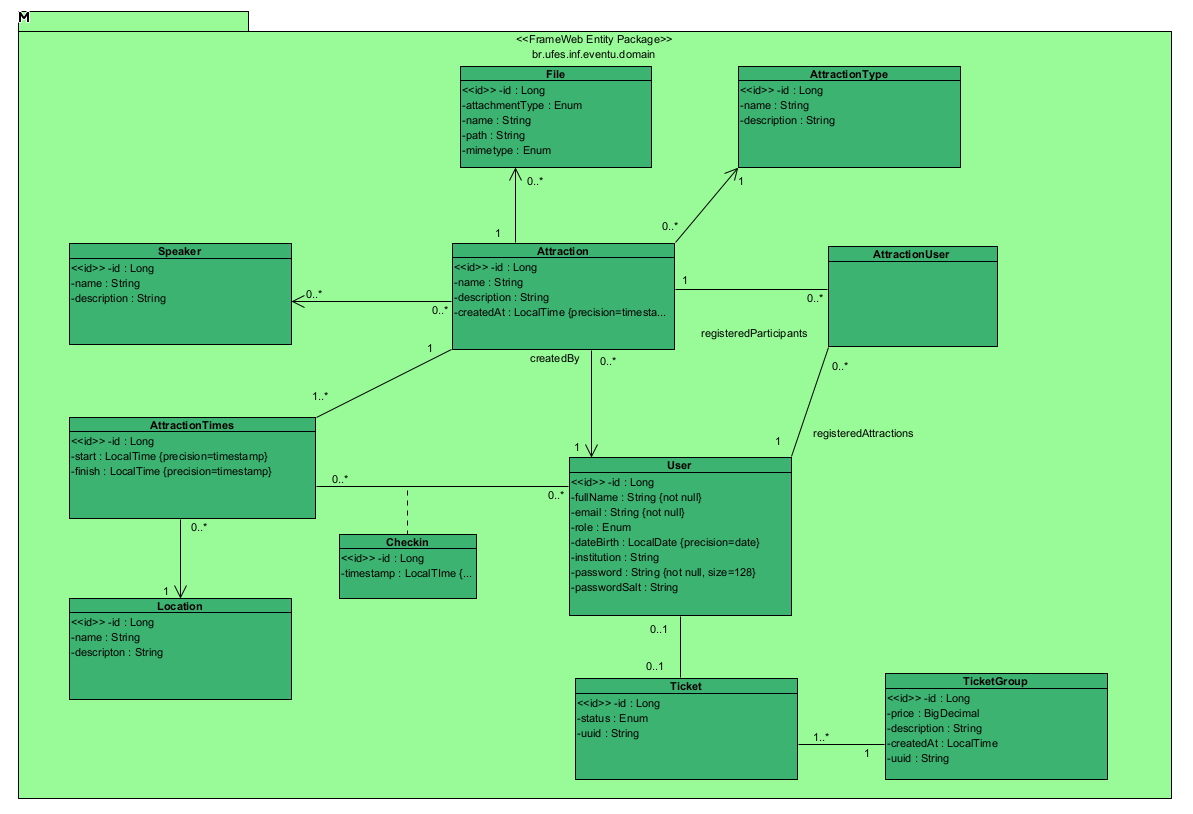
\includegraphics[width=0.8\textwidth]{figuras/ClassesDeDominio.PNG}
	\caption{Modelo de Entidades.}
	\label{figura-dominio}
\end{figure}

\textbf{Attraction}: Representa uma atração em um evento, como palestra, workshop ou visita técnica.

\textbf{Speaker}: Representa um palestrante ou outro profissional que participará de uma atração.

\textbf{File}: Representa um arquivo armazenado no sistema, como material de apresentação ou foto.

\textbf{AttractionType}: Representa o tipo de atração, como palestra, workshop ou visita técnica.

\textbf{User}: Representa um usuário do sistema, como participante, organizador ou staff.

\textbf{Ticket}: Representa um ingresso para um evento, com informações como tipo de ingresso, valor e local.

\textbf{TicketGroup}: Representa um grupo de ingressos, permitindo a emissão de vários ingressos de uma vez com um identificador comum.

\textbf{CheckIn}: Classe de relacionamento entre o horario da atração e um usuário, utilizada para registro de presença.

\textbf{CheckIn}: Classe de relacionamento entre o horario da atração e um usuário, utilizada para registro de presença.

Também foram usadas classes de enumeração (\textit{Enums}) para listar valores possíveis de algumas classes como \textbf{Role}, que representa o papel do usuário no sistema, \textbf{AttachmentType}, que representa o tipo de anexo que foi associado à uma atração e \textbf{TicketStatus}, que representa os possíveis status de um ingresso que foi emitido.

\section{Modelo De Aplicação}
\label{sec-frameweb-app}


\begin{figure}[h]
	\centering
	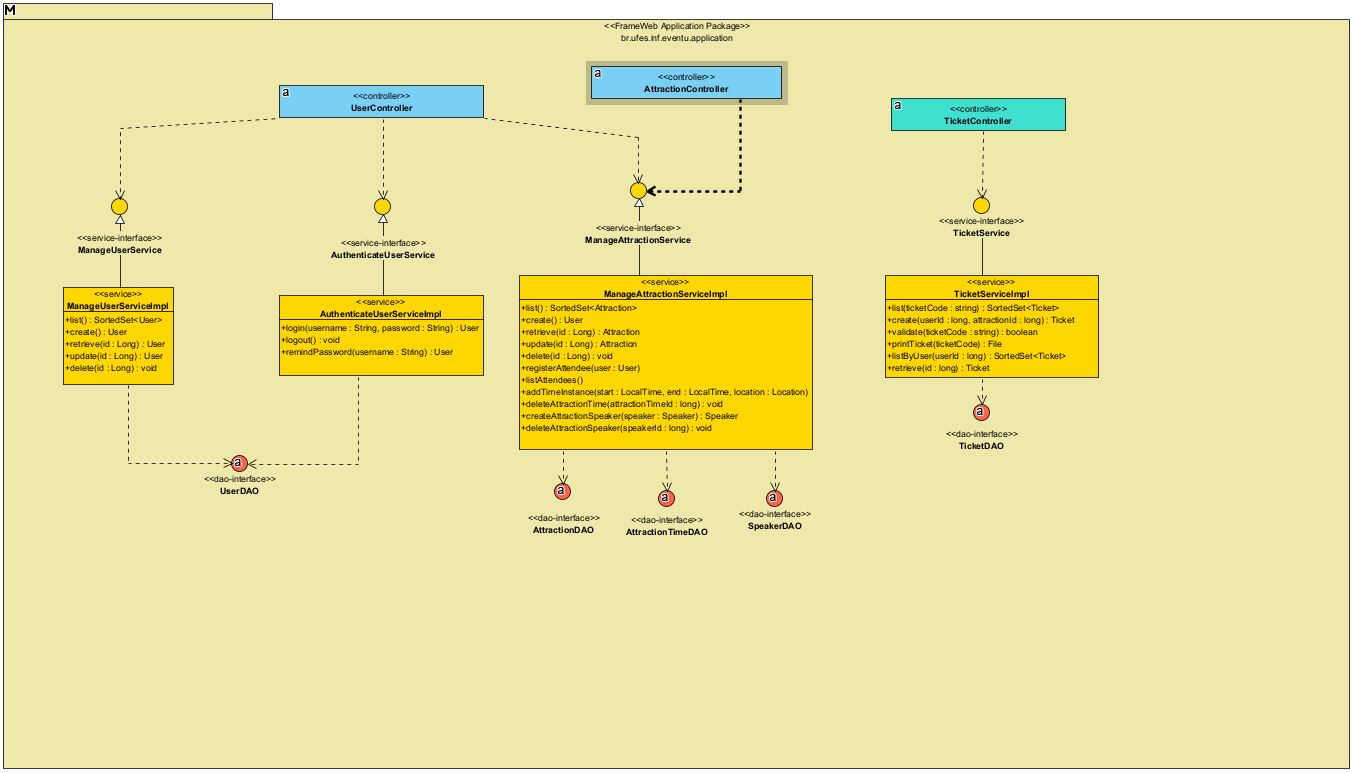
\includegraphics[width=0.8\textwidth]{figuras/ModeloAplicacao.PNG}
	\caption{Modelo de Aplicação.}
	\label{figura-app}
\end{figure}


\section{Camada de Acesso a Dados}
\label{sec-frameweb-dados}


\begin{figure}[h]
	\centering
	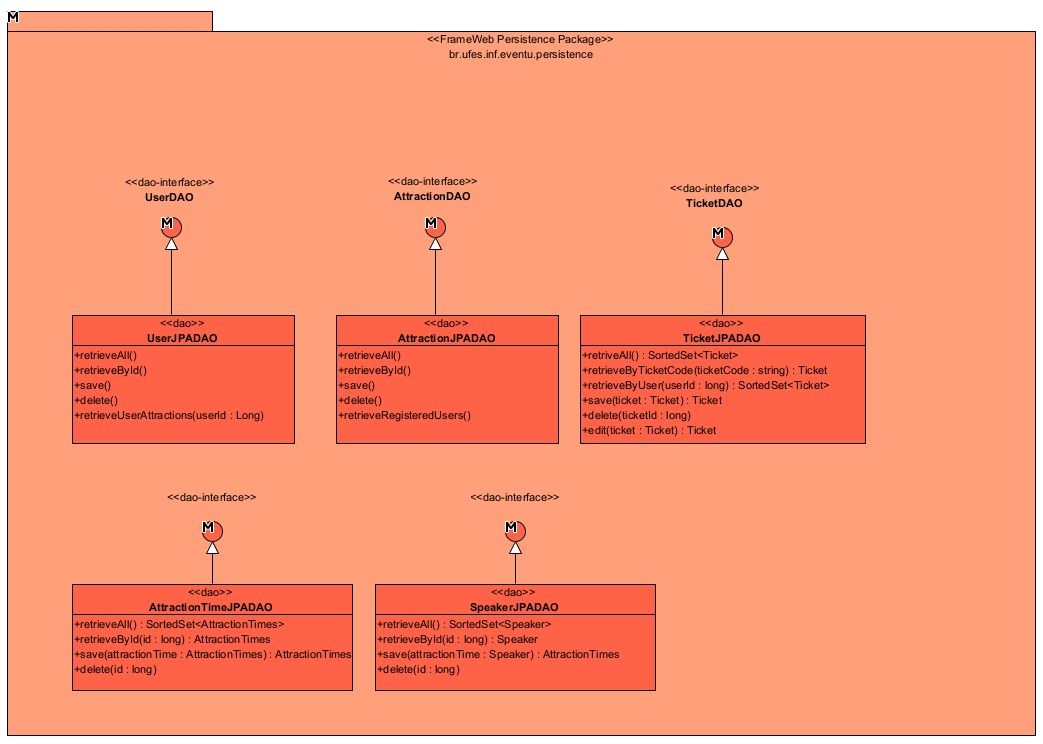
\includegraphics[width=0.8\textwidth]{figuras/ClassesDePersistencia.PNG}
	\caption{Modelo de Persistencia.}
	\label{figura-persistencia}
\end{figure}

Além das funcionalidades CRUD (do inglês: Criação, Consulta, Atualização e Destruição) herdadas da classe \textit{org.springframework.data.jpa.repository.JpaRepository}, podemos ressaltar na camada de acesso a dados algumas outras operações:

\textbf{TicketJPADAO}: +retireveByTicketCode - Operação responsável por encontrar o ticket no banco de dados durante o processo de validação do ingresso.

\textbf{AttractionJPADAO}: +retireveRegisteredUsers() - Operação responsável por retornar a lista de usuários inscritos em uma dada atração.


\section{Camada de Apresentação}
\label{sec-frameweb-apresentacao}

\begin{figure}[h]
	\centering
	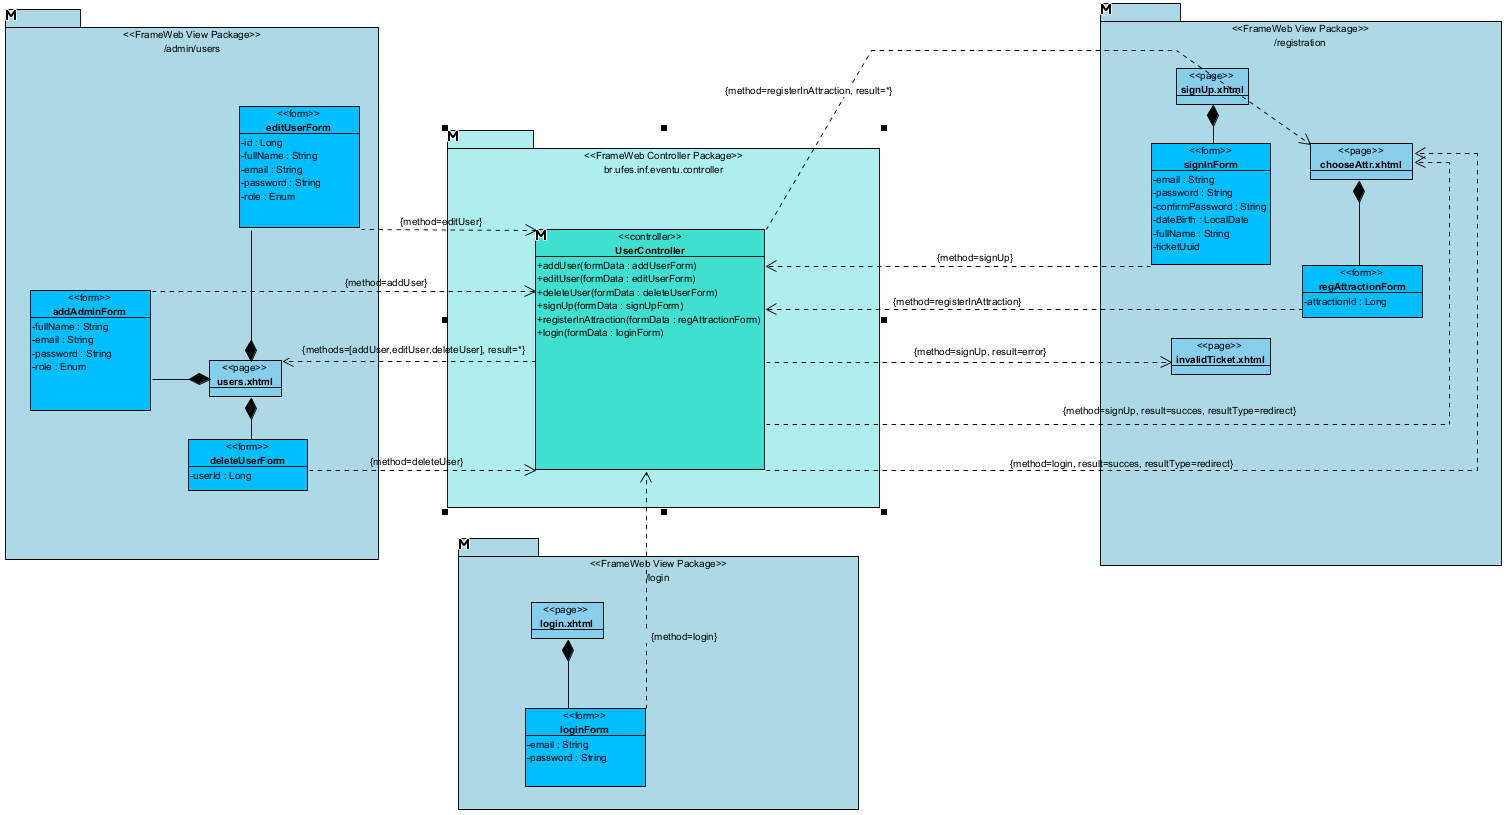
\includegraphics[width=0.8\textwidth]{figuras/ModeloNavegacaoUser.PNG}
	\caption{Modelo de Navegação - Cadastro de Usuários.}
	\label{figura-cadastrouser}
\end{figure}

A camada de apresentação é responsável pelas diversas telas do sistema. na Figura \ref{figura-cadastrouser} vemos o 3 fluxos de navegação envolvendo usuários.

Em \textbf{/admin/users} vemos o processo de gestão dos usuários por administradores.

Em \textbf{/registration} vemos o cadastro de usuários, criação de login e senha, além da validação do ticket que é comprado fora do sistema. O sistema apenas faz validação do código e a associação ao usuário. Após isso, o usuário e apresentado à tela \textbf{chooseAttr.xhtml} em que ele escolhe progressivamente  as atrações que vai participar.

Em \textbf{/registration} vemos o cadastro de usuários, criação de login e senha, além da validação do ticket que é comprado fora do sistema. O sistema apenas faz validação do código e a associação ao usuário. Após isso, o usuário e apresentado à tela \textbf{chooseAttr.xhtml} em que ele escolhe progressivamente  as atrações que vai participar.

Em \textbf{/login} vemos o fluxo de autenticação do usuário.

\begin{figure}[h]
	\centering
	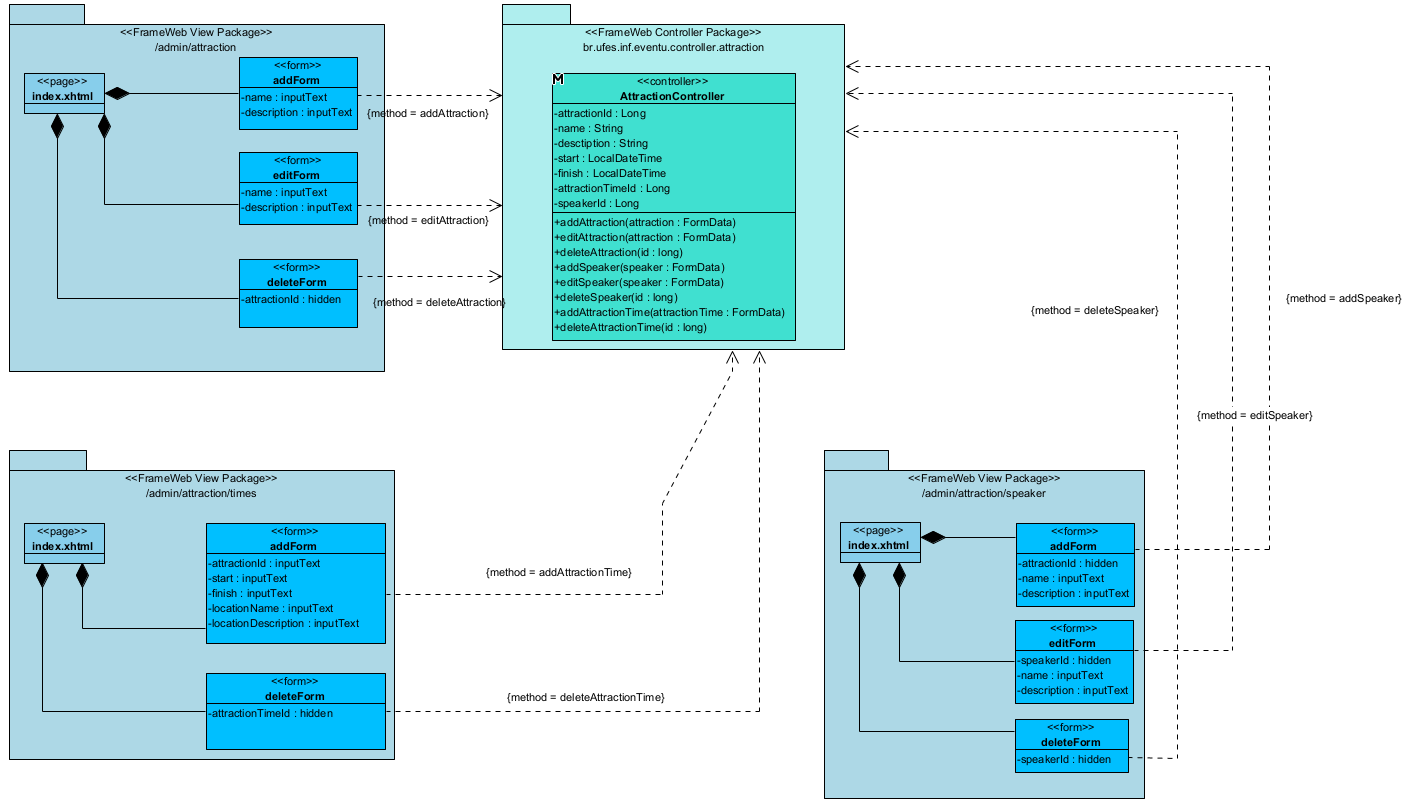
\includegraphics[width=0.8\textwidth]{figuras/ModeloNavegacaoAttr.PNG}
	\caption{Modelo de Navegação - Cadastro de Atrações.}
	\label{figura-cadastroattr}
\end{figure}


Na Figura \ref{figura-cadastroattr} vemos mais 3 fluxos de navegação, agora envolvendo envolvendo o cadastro de atrações.

O processo se assemelha a um simples CRUD, assim como na gestão de usuários por administradores. O ponto a ressaltar é que as atrações estão relacionadas à entidade palestrante e as instâncias de horário. Instancias de horário foram modeladas dessa forma para acomodar atrações que se estendam por mais de um dia, em locais diferentes. Para isso temos a classe \textit{AttractionTimes}
 
\begin{figure}[h]
	\centering
	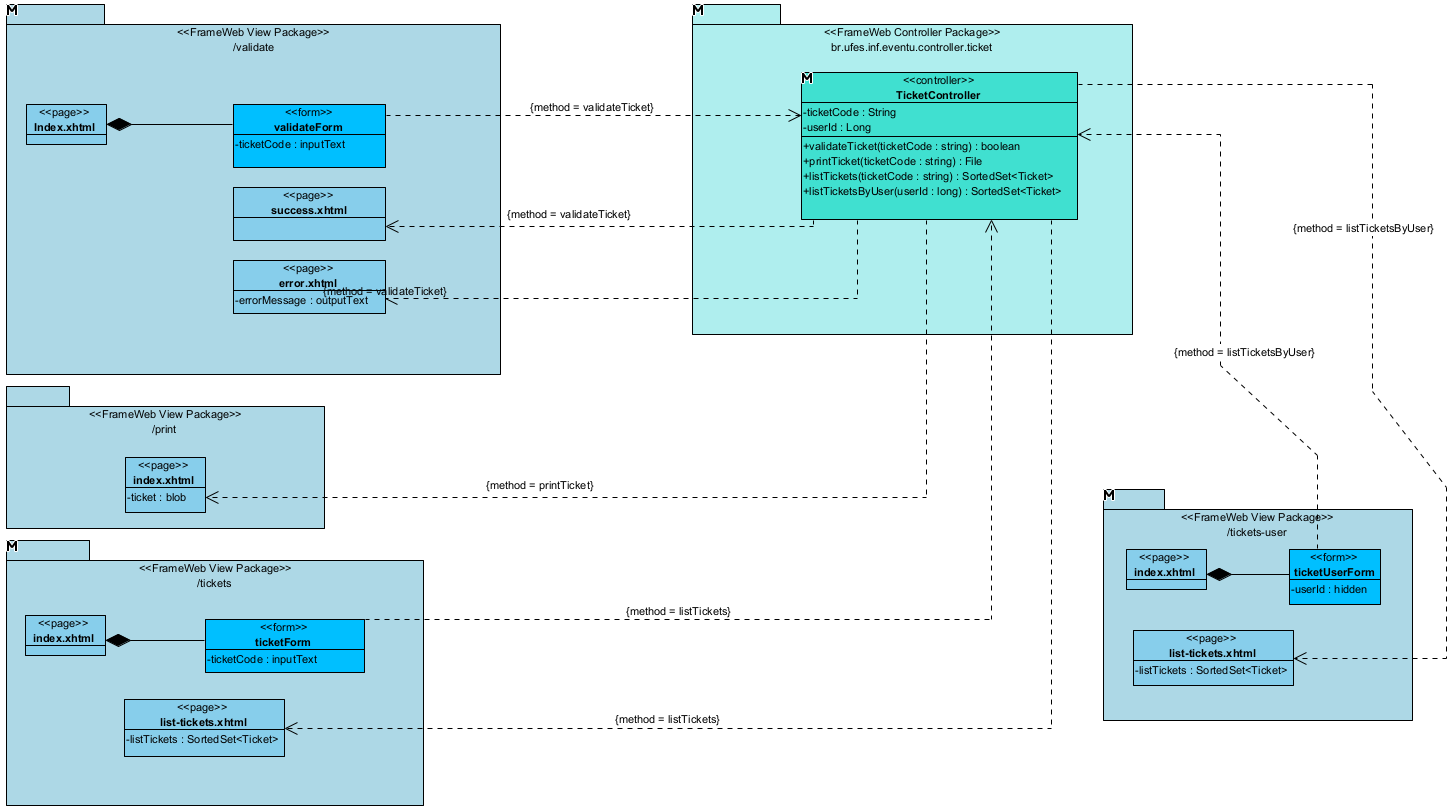
\includegraphics[width=0.8\textwidth]{figuras/ModeloNavegacaoTicket.PNG}
	\caption{Modelo de Navegação - Cadastro de Tickets.}
	\label{figura-cadastrotickets}
\end{figure}

Na Figura \ref{figura-cadastrotickets} vemos mais 4 fluxos de navegação, desta vez envolvendo envolvendo os ingressos (\textit{Tickets}).

O ponto interessante de se ressaltar é a operação \textbf{+printTicket()} que permite um administrador imprimir um ingresso, facilitando a emissão para venda física.